\section{Signal extraction}
\label{Signal extraction}
The numbers of prompt and from-$b$ \jpsi and \psitwos signal candidates are extracted from a simultaneous fit to the invariant mass and pseudo-proper time $t_z$ distributions. For prompt production, $t_z$ is equal to 0 while for charmonium coming from the decay of a $B$ hadron, $t_z$ is a good approximation of the $B$ hadron propertime and should follow an exponential distribution.

\subsection{Mass fit function}
The procedure that is described in the following is very close to the one used in previous $pp$ analyses~\cite{LHCb:2015foc}. The function describing the invariant mass of the signal candidates is a Crystal Ball function defined in Eq.~\ref{CBfunction}.
\begin{equation}
 f_{\mathrm{CB}}(m;\mu,\sigma,\alpha,n) =
 \begin{cases}
      \Big(\frac{n}{|\alpha|}\Big)^n e^{-\frac{1}{2}\alpha^2} (\frac{n}{|\alpha|}-|\alpha|-\frac{m-\mu}{\sigma})^{-n} & \frac{m-\mu}{\sigma} < -|\alpha|\\
   \exp\Bigg( -\frac{1}{2}\Big(\frac{m-\mu}{\sigma}\Big)^2\Bigg) & \frac{m-\mu}{\sigma}>-|\alpha|.
\end{cases}.
\label{CBfunction}
\end{equation}
The value of the parameter n is fixed to 1 following the physics arguments described in Ref.~\cite{LefrancoisTalk}, while the value of the parameter $\alpha$ is constrained from the values of the resolution parameter $\sigma$ following
\begin{equation}
\alpha = 2.066+0.0085\sigma-0.00011\sigma^2,
\label{alphasigma}
\end{equation}
 extracted from toy Monte Carlo studies and where $\sigma$ is expressed in \mev. The background, which is only combinatorial, is described by an exponential function,
\begin{equation}
f_{bkg}(x;p)=e^{-px}.
\end{equation}
For \jpsi mass fit, two crystal ball function with common mean value are applied to describe the signals while for \psitwos, only one is used.
\subsection{Pseudo-propertime fit function}
To determine the signal yields of prompt and from-\bquark components separately, the $t_z$ distribution is used. In each kinematic and multiplicity bin, an unbinned extended maximum likelihood fit to the two-dimension distributions of invariant mass $m(\mumu)$ and $t_z$ is performed to separate prompt component from that from \bquark.
At the generator level, the $t_z$ distribution of the prompt component is a Dirac delta function, $\delta(t_z)$, while that from $\bquark$ follows an exponential function as seen from simulation. For \jpsi and \psitwos signals, the detector resolution is taken into account by convolving a resolution function, which is described by the sum of two Gaussian functions with a common mean and resolution parameters $\sigma$ and $2\sigma$ respectively:
\begin{equation}
f_\mathrm{resolution}(t_z;\mu,\sigma,\beta) = \frac{\beta}{\sqrt{2\pi}\sigma} e^{-\frac{(t_z-\mu)^2}{2\sigma^2}}
+\frac{1-\beta}{2\sqrt{2\pi}\sigma} e^{-\frac{(t_z-\mu)^2}{8\sigma^2}}.
\end{equation}
The background control sample consists of random combinations of muons from semi-leptonic $\bquark$ and $\cquark$ decays, which tend to produce positive $t_z$ values, as well as mis-reconstructed tracks from decays-in-flight of kaons and pions, which contribute both to positive and negative $t_z$ values. The $t_z$ distribution of the background is therefore modeled with an empirical function, composed of a Dirac delta function and five exponentials (three for positive $t_z$ and two for negative $t_z$, with one positive $t_z$ and one negative sharing the same slope parameter). This function is convolved with the sum of two Gaussian functions as a resolution function, which has different parameters as for signals. The fit function for $t_z$ background is as follows,
\begin{align}
f_\mathrm{background} &=
\left[(1-f_1-f_2-f_3-f_4)\delta(t_z)+\theta(t_z)(\frac{f_1}{\tau_1}e^{-t_z/\tau_1}+\frac{f_2}{\tau_2}e^{-t_z/\tau_2})\right.
\nonumber\\
&\left. +\theta(-t_z)\frac{f_3}{\tau_3}e^{t_z/\tau_3}+\frac{f_4}{2\tau_4}e^{-|t_z|/\tau_4}
\right]\ast \left(\frac{\beta'}{\sqrt{2\pi}S^{'}_1\sigma} e^{-\frac{(t_z-\mu)^2}{2S^{'2}_1\sigma^2}}
  +\frac{1-\beta'}{\sqrt{2\pi}S^{'}_2\sigma} e^{-\frac{(t_z-\mu)^2}{2S^{'2}_2\sigma^2}}\right).
\label{eq:TzBKG}
\end{align}
The shape of the background is chosen empirically based on the shape seen in the $t_z$ distribution of the \jpsi and \psitwos mass side-bands, which are at 50 \mevcc away from the mass values from the PDG.
The fit procedures are as follows,
\begin{itemize}
\item First step, the one-dimensional fit to the mass spectrum is performed to estimate the yield and the parameters of inclusive (sum of prompt and from-$b$) signal candidates, the background yield and of the exponent of the background function.
\item Second step, the mass sideband candidates ($|M-M^{PDG}|>50\mevcc$) are used to fit the $t_z$ distribution for the background. 
\item Last step, a simultaneous fit to the mass and the pseudo-proper decay time distributions is then performed.
\end{itemize}

As examples, the $t_z$ background fit for \jpsi and \psitwos are shown in Figure~\ref{fig_tzbkg} for $4\leq N_{\rm tracks}^{\rm PV} < 45$ in $p$Pb  configurtion and the 2-dimensional fit projected in mass spectrum and $t_z$ spectrum are shown in Figure~\ref{fig_2DFit} for $4\leq N_{\rm tracks}^{\rm PV} < 45$ in  $p$Pb configuration. The fit results for other multiplicity class in $p$Pb and Pb$p$ configurations can be found in appendix.
\begin{figure}[!tbp]
\begin{center}
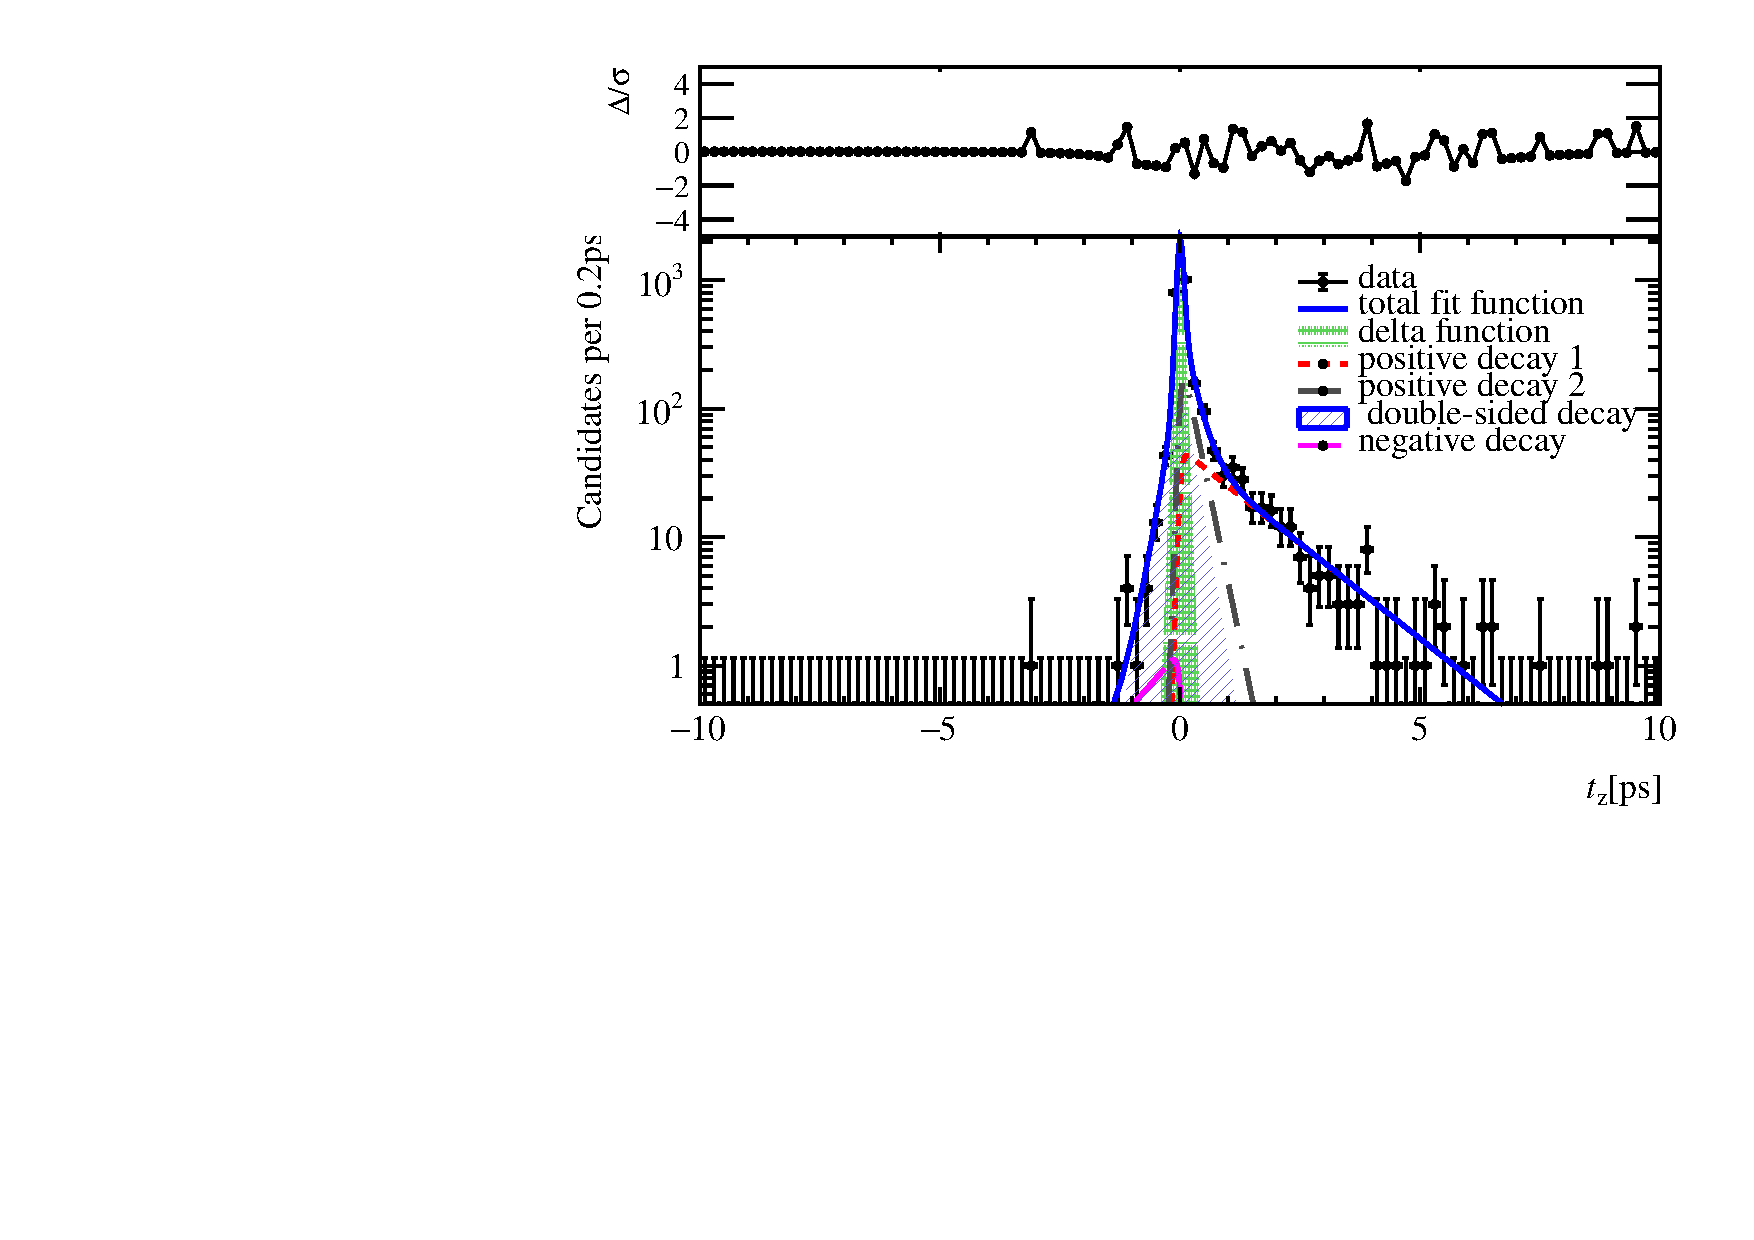
\includegraphics[width=0.49\linewidth]{pdf/pPb/Workdir/TzbkgFit/Jpsi_n1y1pt1.pdf}
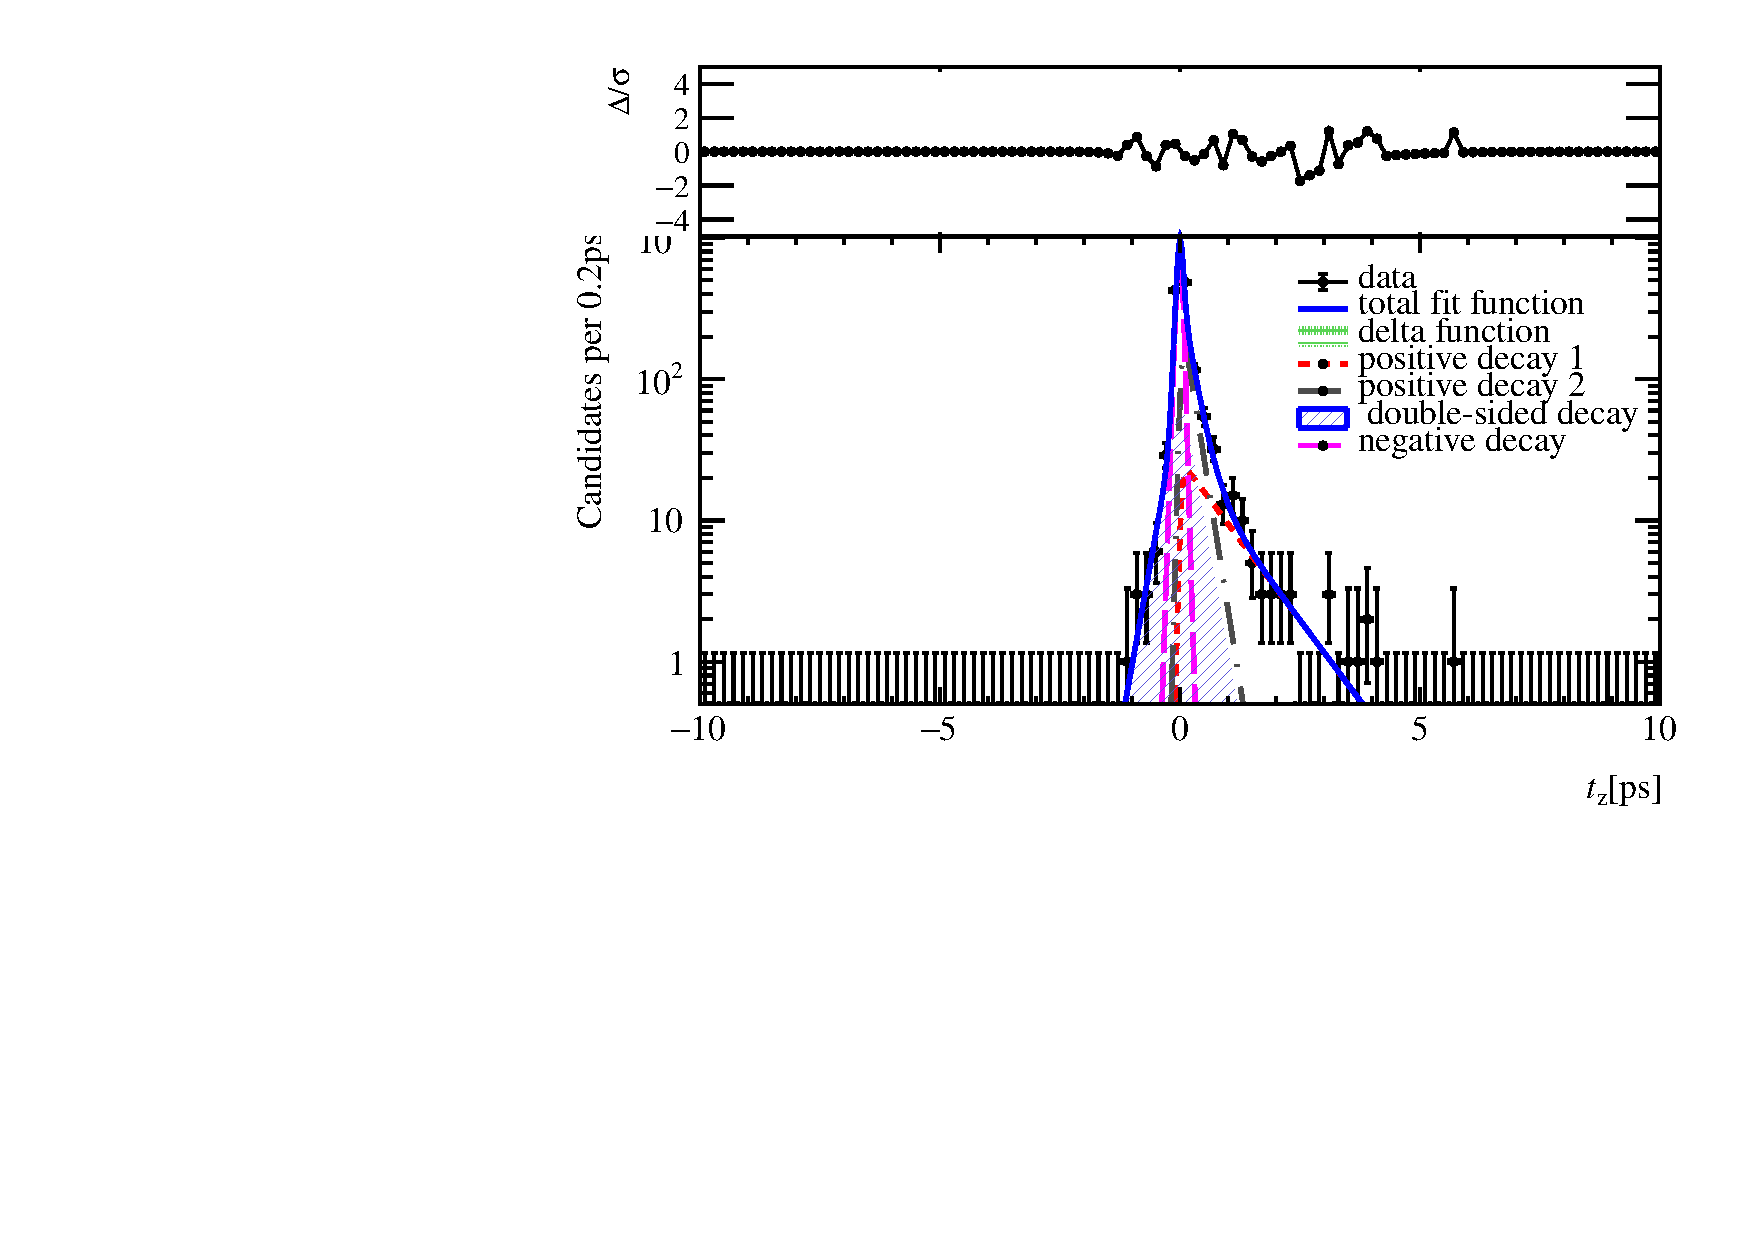
\includegraphics[width=0.49\linewidth]{pdf/pPb/Workdir/TzbkgFit/Psi2S_n1y1pt1.pdf}
\end{center}
\caption{
	$t_z$ background fit for \jpsi (left) and \psitwos (right) for $4\leq N_{\rm tracks}^{\rm PV} < 45$ in $p$Pb configuration.}
\label{fig_tzbkg}
\end{figure}
\begin{figure}[!tbp]
\begin{center}
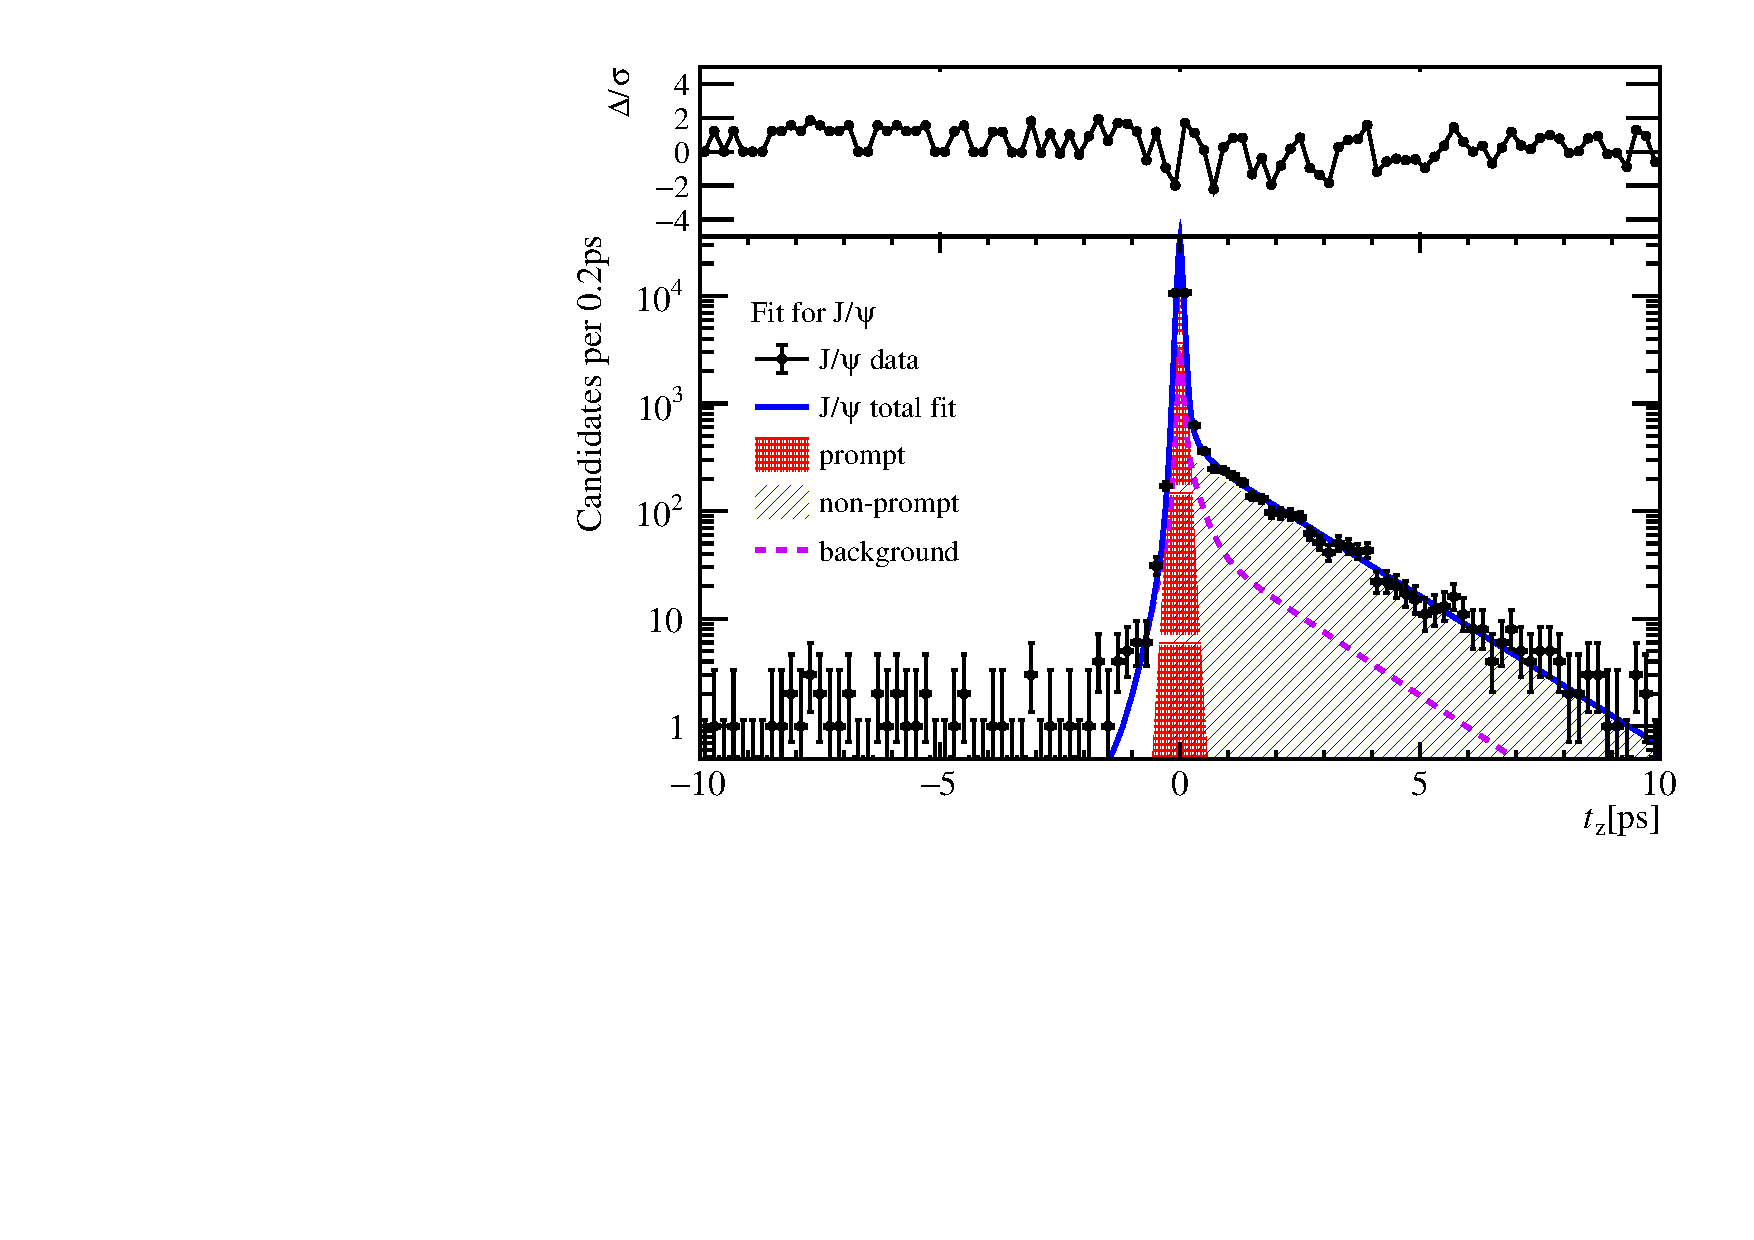
\includegraphics[width=0.49\linewidth]{pdf/pPb/Workdir/TwoDimFit/ProjTz/Jpsi_n1y1pt1.pdf}
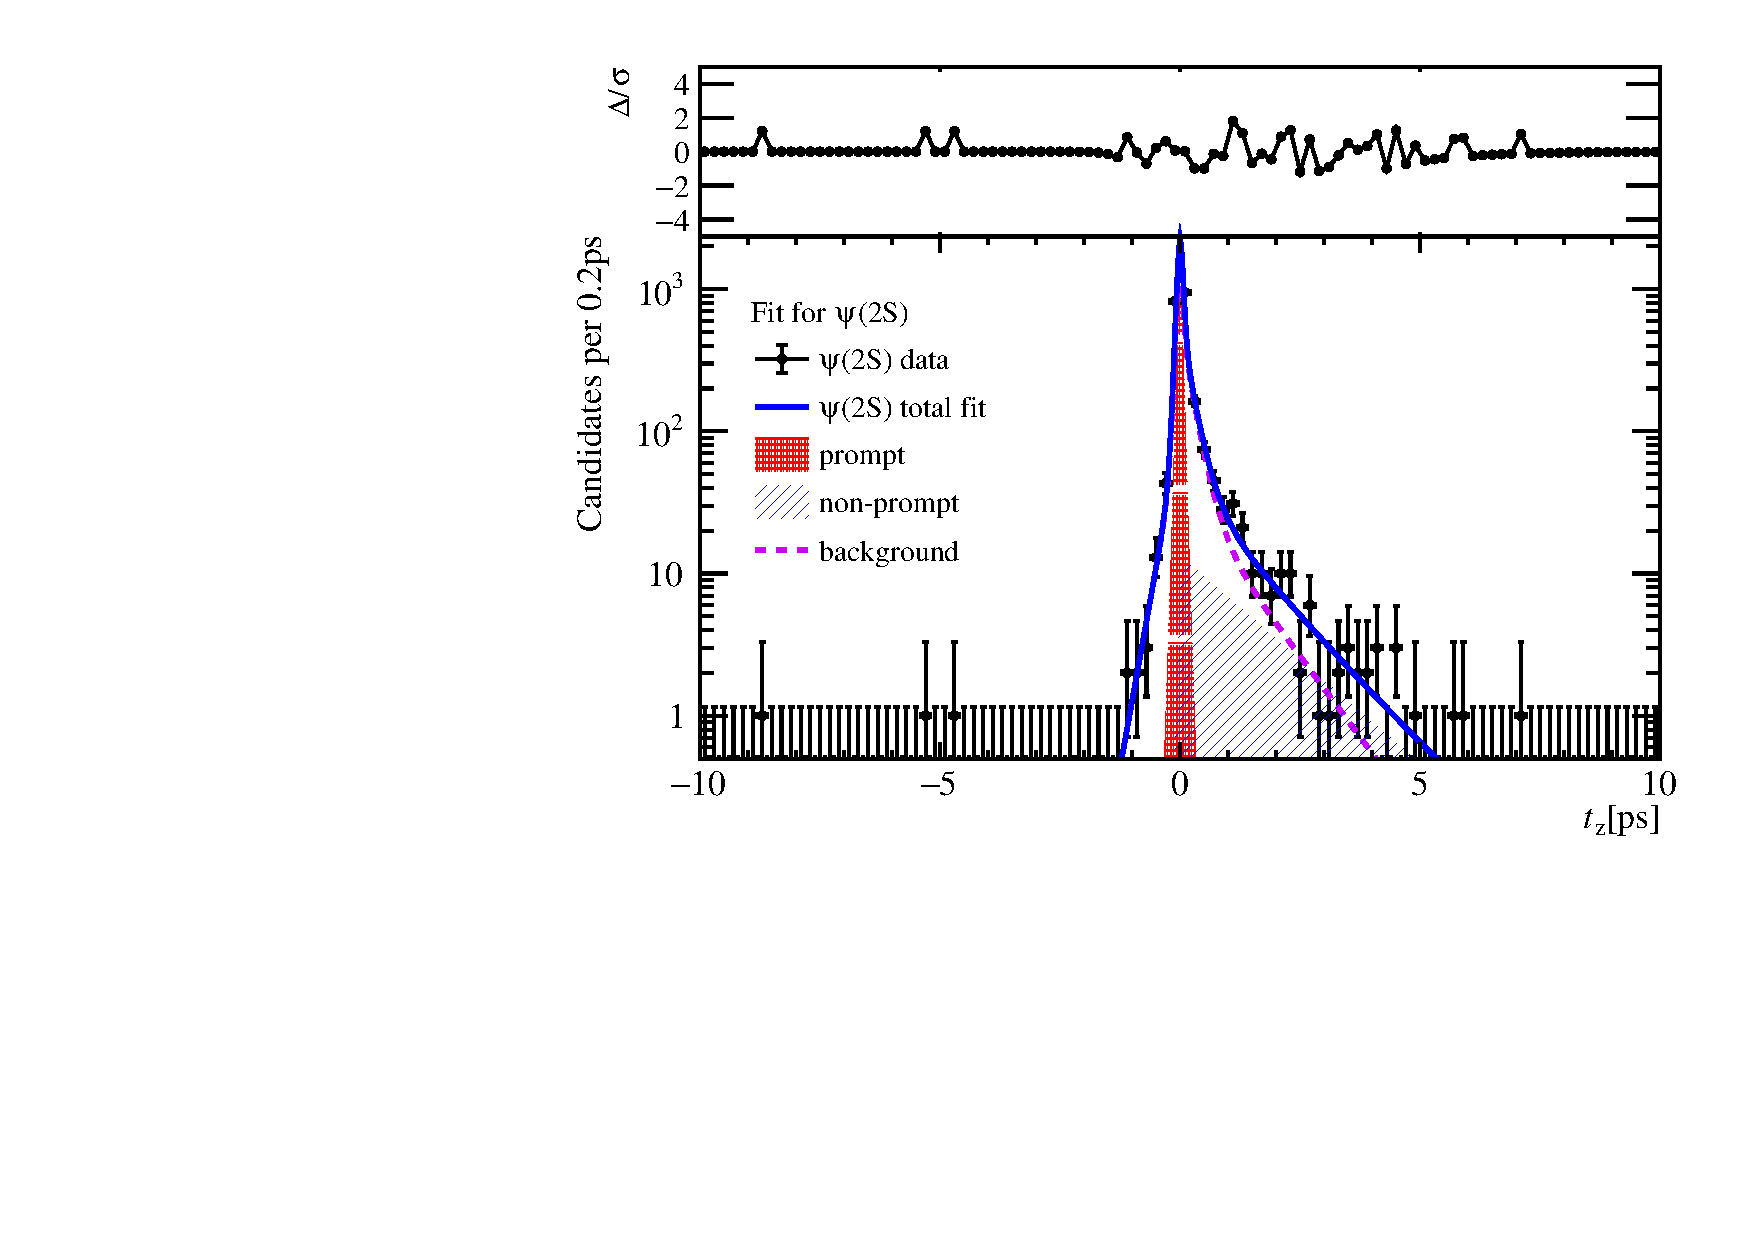
\includegraphics[width=0.49\linewidth]{pdf/pPb/Workdir/TwoDimFit/ProjTz/Psi2S_n1y1pt1.pdf}
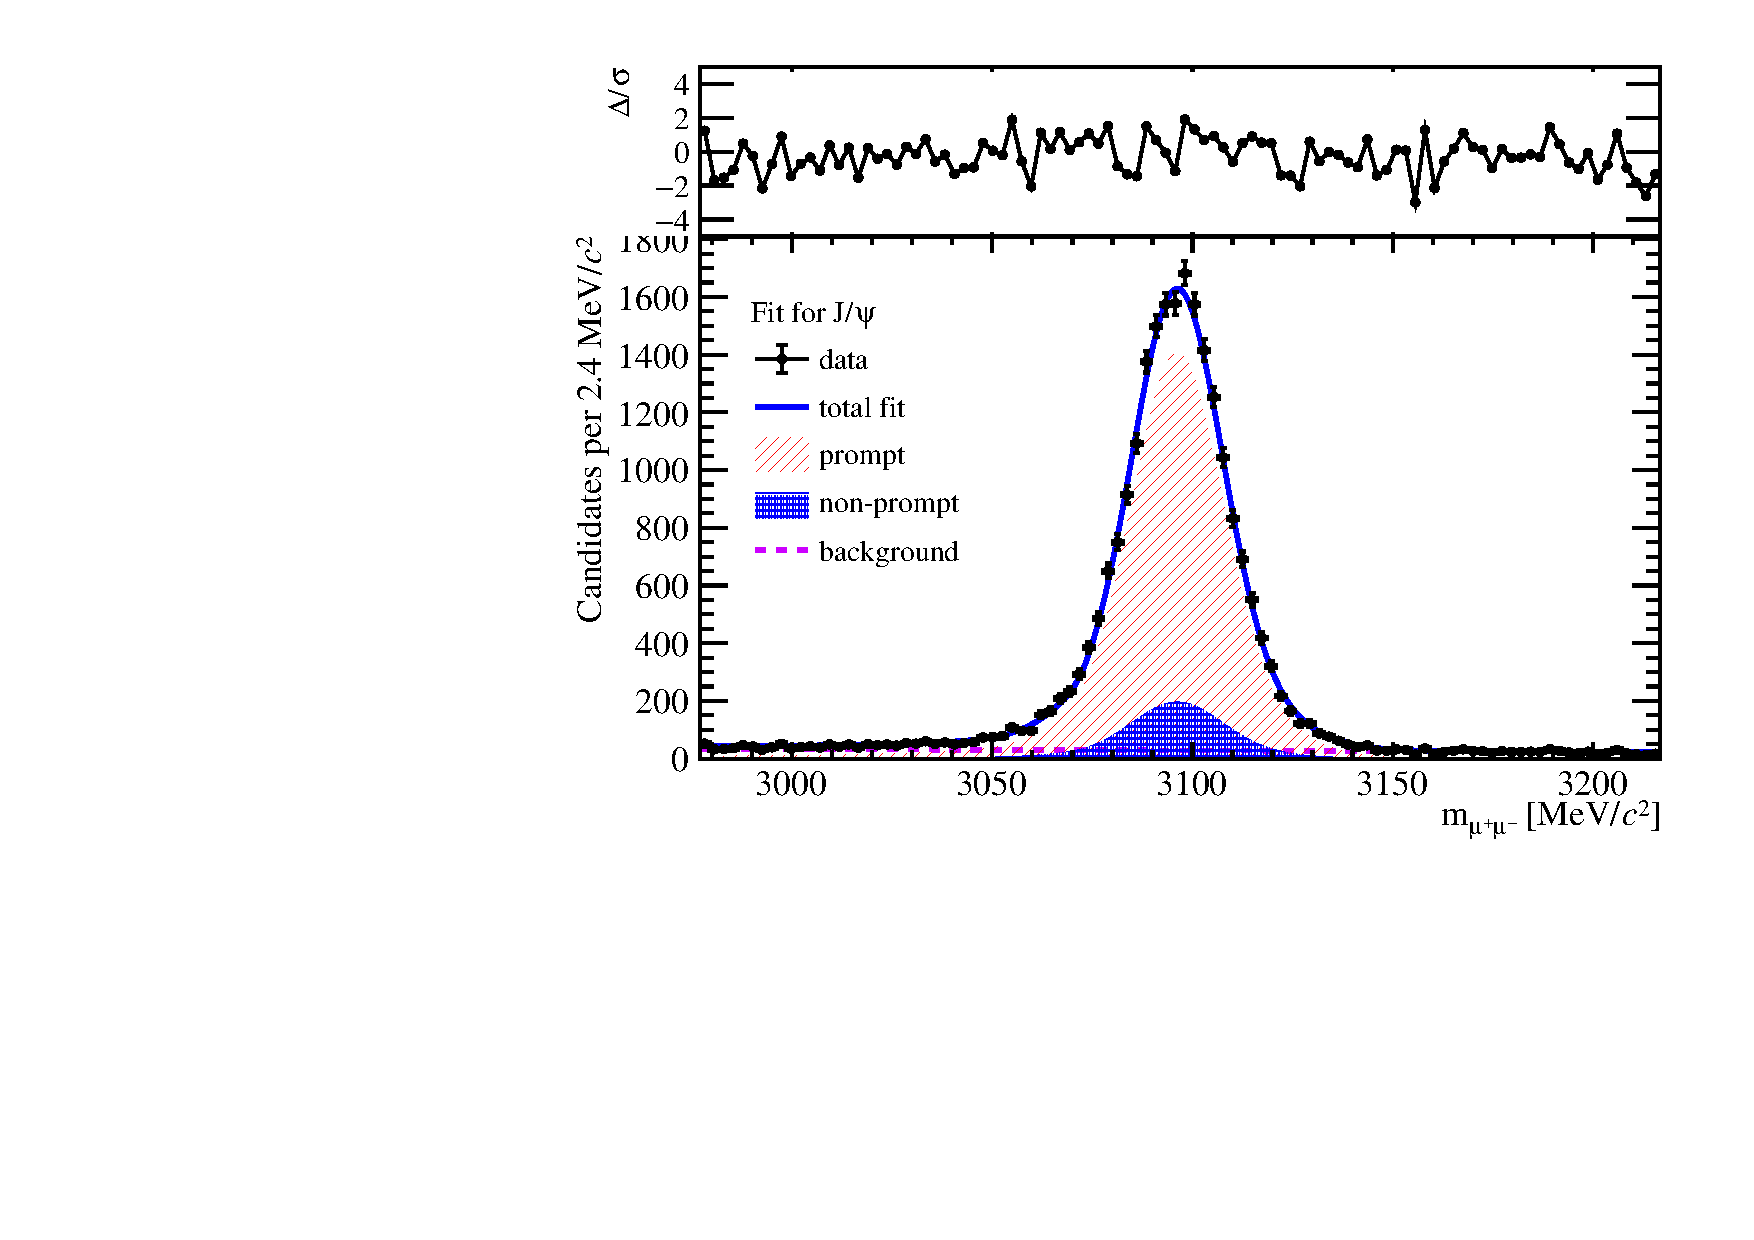
\includegraphics[width=0.49\linewidth]{pdf/pPb/Workdir/TwoDimFit/ProjMass/Jpsi_n1y1pt1.pdf}
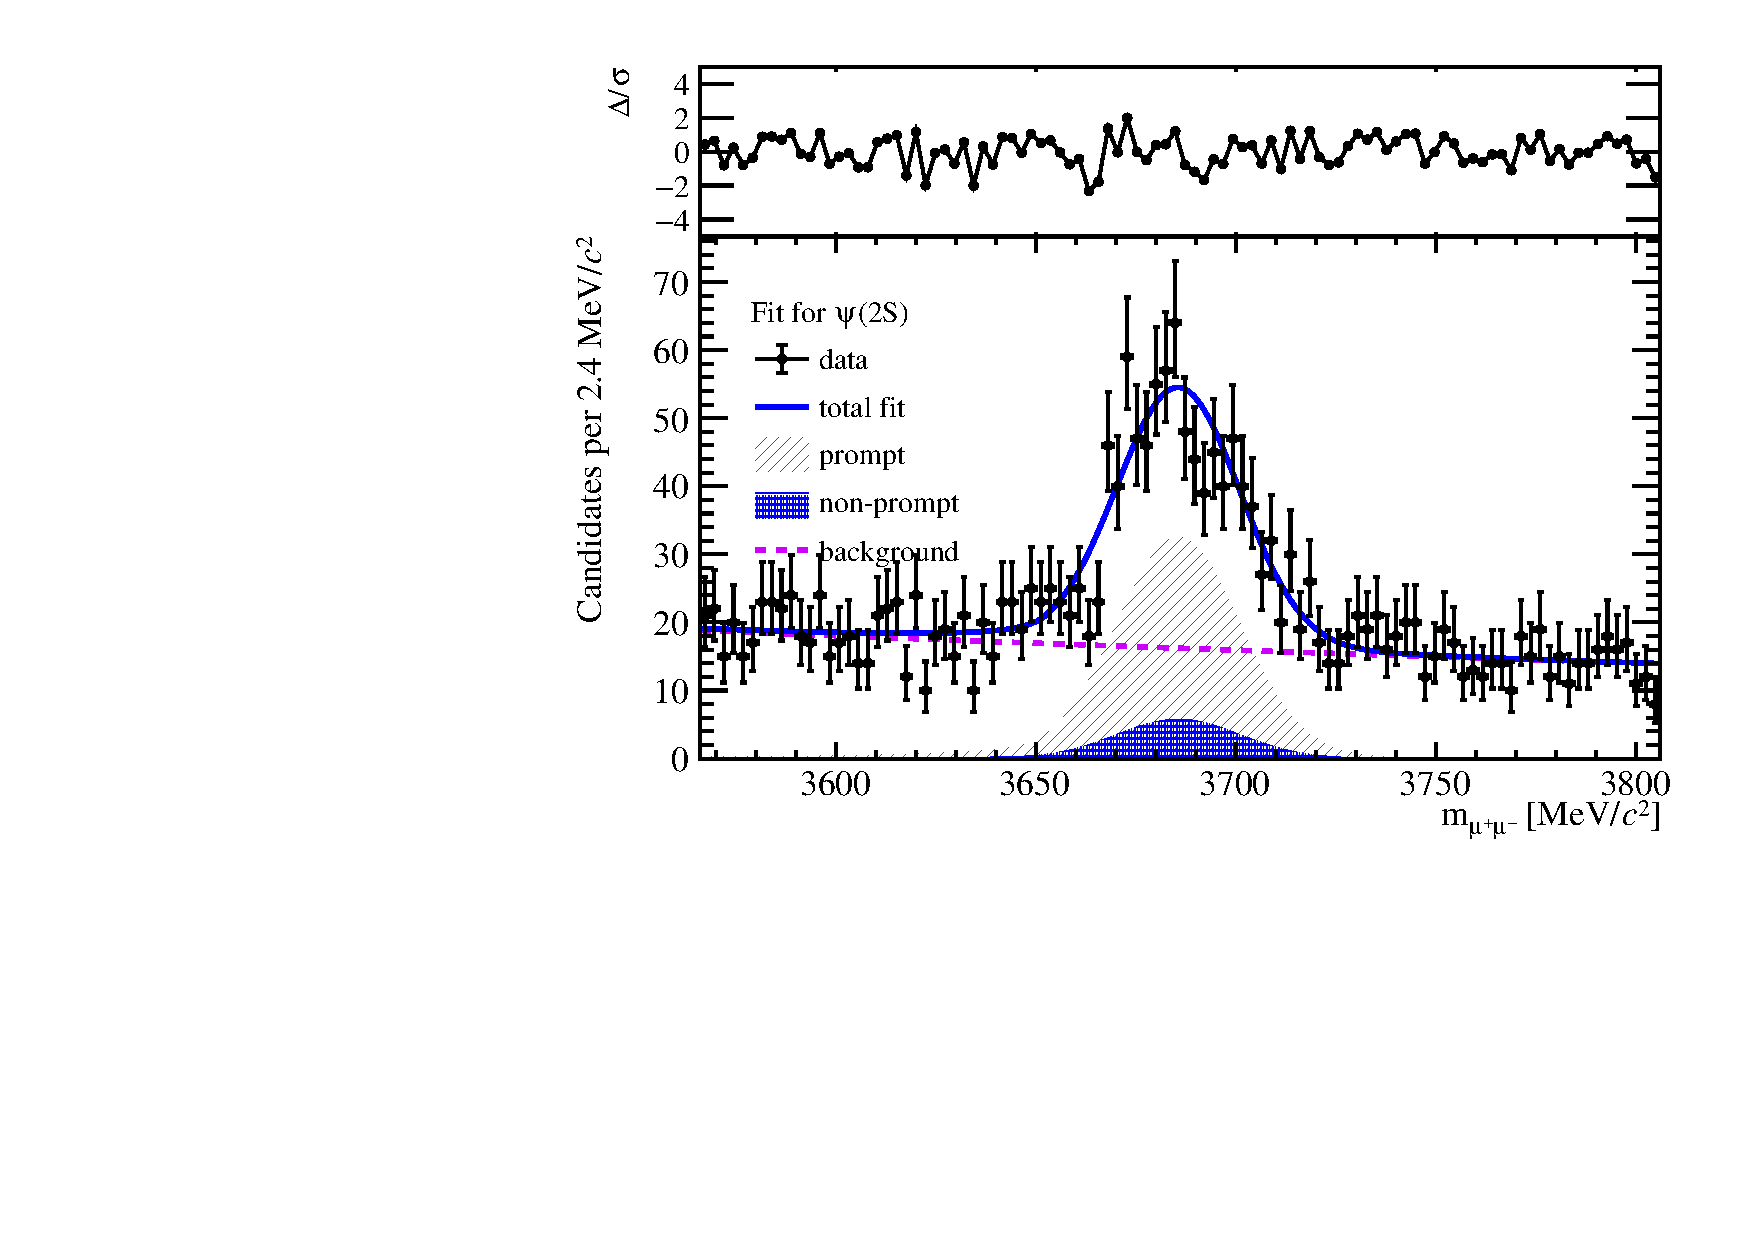
\includegraphics[width=0.49\linewidth]{pdf/pPb/Workdir/TwoDimFit/ProjMass/Psi2S_n1y1pt1.pdf}
\end{center}
\caption{
	2-Dimensional fit projected on $t_z$ spectrum (first row)  and mass spectrum (second row) for \jpsi (left) and \psitwos (right) for $4\leq N_{\rm tracks}^{\rm PV} < 45$ in $p$Pb configuration.}
\label{fig_2DFit}
\end{figure}
